% !TeX spellcheck = english
% !TEX root = thesis.tex
\section{Methods and Materials}
\label{ch:Exp}

    \subsection{\hlr{Fabrication of Nanoparticles by Femtosecond Laser Ablation}}
    \label{sec:Ablation}
%            The first part of the project was to develop a new, simple, method of fabricating crystalline dielectric
%        nanoparticles. The idea was to use controlled laser ablation~--- a very simple technique~--- to produce the particles.
%        Previous work on the topic by us [PARTICLE WRITING] and Boris Chichkov [LASER PRINTING] gave two methods that could be
%        adapted to our needs. Our method, laser writing, had been used to fabricate large-scale arrays of plasmonic particles,
%        and could, in theory be adapted to dielectric particles. Boris Chichkov's laser printing had most of the required
%        characteristics for crystalline particle fabrication - controllable particle size, transfer to other substrates, but
%        was unable to fabricate crystalline particles~--- an additional annealing step was required to crystallize the fabricated
%        particles.

        \begin{figure}[h!]
                \begin{center}
                    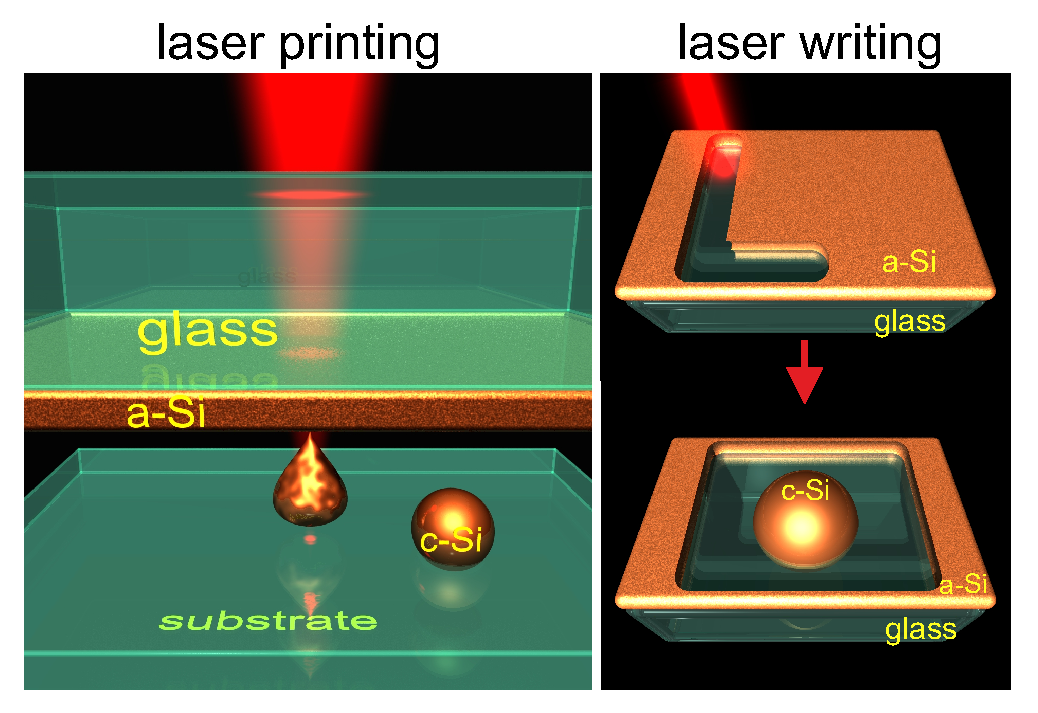
\includegraphics[width=0.5\textwidth]{figs/methods/LaserPrinting.eps}
                \end{center}
                \label{fig:LaserPrinting}
                \caption{Geometry of laser-ablation based fabrication methods of crystalline nanoparticles from amorphous
                            thin films.}
        \end{figure}


        \subsubsection{\hlr{Laser writing of dielectric particles}}
                The novel method of direct laser writing is also applicable for c-Si nanoparticles fabrication from initially amorphous
            a-Si:H film. Under the optimal conditions of fabrication the resulting array of nanoparticles has a period of about
            $0.9~\si{\upmu m}$, exhibiting bright colors owing to resonant scattering (figure~\ref{fig:LaserWriting}(a))~\cite{krasnok2015towards}.
            Despite the cutting should produce rectangular grating, our SEM images show the spherical shape of the nanoparticle. Indeed,
            the laser fluence $F\approx100~\si{mJ/cm^{2}}$ provides film heating close to the melting point even in a single shot regime,
            whereas $12.5~\si{ns}$ delay between pulses leads to the temperature accumulation and exceeding of the ablation threshold.
            The heat transferring from the ablated area to the surrounding film is accumulated much stronger in the cut patches,
            which are thermally isolated from the rest of the film. These micro-patches are unstable at high temperatures and undergo
            dewetting to a certain number of similar nanoparticles~\cite{thompson2012solid}. In order to provide deeper insight,
            we model the time dynamics of the cut liquid Si patch with the height of $80~\si{nm}$ and similar widths of $300~\si{nm}$ (Figs.~\ref{fig:LaserWriting}B)
            on a fused silica substrate in the COMSOL software, solving the incompressible Navier-Stokes equations and taking into account
            the parameters of the used materials. The modeling shows that after ten nanoseconds the patch is transformed into the semisphere with
            the height about $130~\si{nm}$ and width about $310~\si{nm}$ (Figs.~\ref{fig:LaserWriting}B-E), giving qualitative agreement with
            the experimentally observed shapes.



        \subsubsection{\hlr{Laser transfer of crystalline dielectric particles}}
                The silicon nanoparticles  were printed by a femtosecond laser system (Femtosecond Oscillator TiF-100F, Avesta Poject),
            which emits laser pulses at a central wavelength of $800~\si{nm}$, with pulse duration of $100~\si{fs}$, and repetition rate
            of $80~\si{MHz}$. Laser pulses selected by a Pockels cell-based pulse picker (Avesta Poject) were tightly focused by an
            oil immersion microscope objective (Olympus $100\times$) with a numerical aperture of $\mathit{NA}=1.4$. According to the
            relation $\emph{d}\approx 1.22\lambda/\mathit{NA}$, the estimated diameter of the beam's focal spot size is $d=0.7~\si{\upmu m}$,
            close to the value measured by a method based on the dependence of the laser-damaged area on incident laser energy ($0.68~\si{\upmu m}$)~\cite{liu1982simple}.
    	    The nanoparticles were fabricated from an $80~\si{nm}$ thick a-Si:H film, which was deposited on a substrate of fused silica by
            plasma enhanced chemical vapor deposition from a SiH$_{3}$ precursor gas. The samples were placed on a three-dimensional air-bearing
            translating stage driven by brushless servomotors (ABL1000, Aerotech), with sample translation accuracy at least $100~\si{nm}$.
	        The nanoparticles were fabricated by single laser pulses (from a previously undamaged surface) in the forward-transfer geometry,
            in which the receiving substrate is placed under the film with a spacing of $\sim 50~\si{\upmu m}$ (figure~\ref{fig:LaserPrinting}(a)).
            This geometry has an advantage over the back-transfer geometry owing to the possibility of nanoparticle printing onto a wide
            variety of substrates, including opaque and structured samples. The silicon nanoparticles were printed at laser energies in the
            range of $0.5-1.2~\si{nJ}$, providing fluencies in the range of $0.12-0.16~\si{J/cm^{2}}$. The nanoparticles are almost spherical
            in shape(figure~\ref{fig:Crystallinity}(b)) and their diameters lie in the range of $50-200~\si{nm}$, depending on the fluence.



    \subsection{\hlr{Electron Microscopy and X-Ray Diffractometry}}
    \label{sec:SEM}
            The geometrical parameters of the fabricated particles were measured by Scanning Electron Microscopy (SEM),
        Transmission Electron Microscopy (TEM). X-Ray Diffractormetry was used to probe the crystalline structure of the
        nanoparticles.
        \subsubsection{\hlr{Scanning Electron Microscopy}}
                Indeed, scanning electron microscopy (SEM, Carl Zeiss, Neon 40) confirms that the particles possess \hlr{axial}
            symmetry along the substrate normal (Fig.~\ref{fig:Crystallinity}B). These results correlate with previously observed
            oblateness of printed silicon nanoparticles~\cite{zywietz2014laser}.

        \subsubsection{\hlr{Transmission Electron Microscopy}}
                We used specimen grids (3-mm-diameter, 200-mesh copper grids, coated on one side with a 20-nm-thick film
            of amorphous carbon) to collect nanoparticles ablated from the a-Si:H film. The size, structure, and composition
            of the collected nanoparticles were determined using bright and dark field TEM imaging, see the inset in
            Fig.~\ref{fig:Crystallinity}B. The analysis of the electron diffraction pattern from several nanoparticles shows clear maxima,
            corresponding to certain crystalline planes (Fig.~\ref{fig:Crystallinity}C). \hlr{Because the specimen grids were uneven, the
            nanoparticles were deposited at different angles to the substrate meaning that} TEM imaging also provides infor
            mation on the oblateness of the particles along the direction perpendicular to the substrate surface, giving
            the average ellipticity about $a_{\parallel}/a_{\perp}\approx$1.12, where $a_{\parallel}$($a_{\perp}$) is
            the particle semi-major (semi-minor) axis oriented parallel (perpendicular) to the surface of the substrate.

        \subsubsection{\hlr{X-Ray Diffractormetry}}



    \subsection{\hlb{Optical Measurements}}
            All of the optical characterization measurements were carried out on a multifuncational setup, depicted in
            Fig.~\ref{fig:expSetup}. The setup allowed us to measure optical signals from single nanoparticles, provided that
            there was at least $1\mu$ m between the nanoparticle and its nearest neighbors. The XYZ-stage used for the
            positioning of the particles had $100$nm precision, giving enough control to position a single nanoparticle into
            the center of the excitation beam.

            The scattered light was collected from the top by an objective (Mitutoyo M Plan APO NIR, 100x, NA=0.7),
            sent to a Horiba LabRam HR spectrometer and projected onto a thermoelectrically cooled charge-coupled device
            (CCD, Andor DU 420A--OE 325) with a 150-g/mm diffraction grating. The spectrometer gave us a spectral resolution
            of around $1$nm.

            \begin{figure}[h!]
                    \begin{center}
                        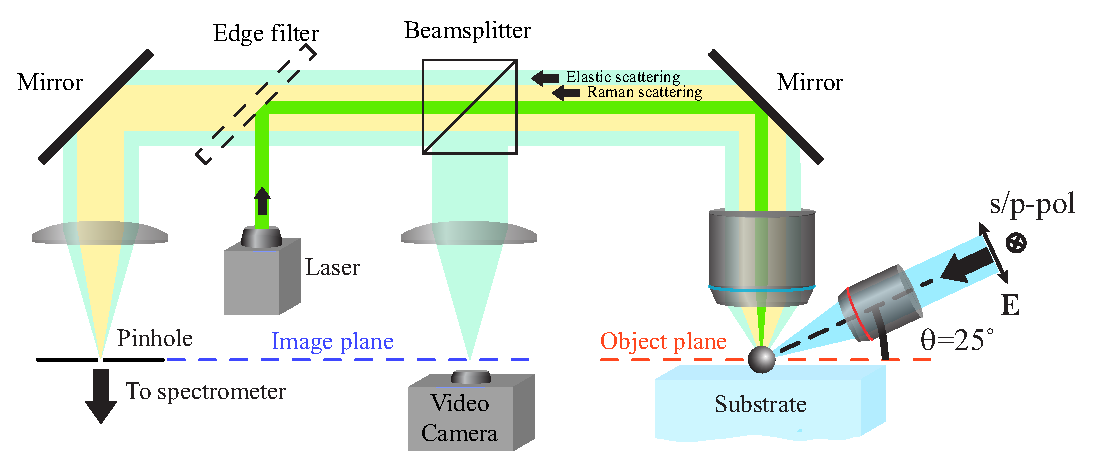
\includegraphics[width=0.9\textwidth]{figs/methods/expSetup2.eps}
                    \end{center}
                    \label{fig:expSetup}
                    \caption{Schematic of the experimental setup used for all of the optical measurements.}
            \end{figure}


        \subsubsection{\hlb{Dark-field Spectroscopy of Single Nanoparticles}}
            \label{sec:Darkfield}
                For the dark-field scattering experiments, the nanoparticles were excited at an oblique angle of incidence
            (65 degrees to the surface normal) by linearly polarized light from a halogen lamp (HL--2000--FHSA)
            through a weakly-focusing objective (Mitutoyo M Plan Apo NIR, 10x, NA=0.28). The polarization allowed us to
            selectively excite different modes in the nanoparticles\cite{permyakov2015probing}.

        \subsubsection{\hlb{Raman Spectroscopy of Single Nanoparticles}}
        \label{sec:Raman}
                For the Raman scattering experiments, the nanoparticles were excited by one of two laser sources: a $632.8$nm HeNe laser
            or a $532$nm Nd:YAG laser, through the same channel that was used to collect the scattered light. A lowpass filter was used
            to filter out the excitaiton wavelength and leave only the Stokes-shifted inelastically scattered light.

    \subsection{\hlb{Numerical Methods}}
    \label{sec:Numeric}
        Several numerical methods were used to simulate the scattering properties of our fabricated nanoparticles~--- to prove their
        crystalline phase, to probe their shape, to determine their size. The initial idea was to use the Discrete Dipole Approximation,
        because it is very flexible and can work with scatterers of arbitrary geometry. The main problem we encountered was the fact
        the method is very involved (especially if one tries to incoroprate substrate interaction), and computationally intensive for
        our problems. Therefore, for most of the calculations presented in this thesis, we used the CST Microwave Studio, which is a
        EM simulation package that uses the Finite Integration Technique for most of its calculations. Being a CAD-based product, it
        allowed us to substantially decrease modelling time for our calculations (even though for such simple calcualtions a simpler
        method would have been more fitting). Also, many calculations turned out to be excessvie~-- a simple Mie theory calculation,
        while simulating the incorrect geometry, was more than enough to model the required parameters, with error well within our
        requirements.

        \subsubsection{\hlb{Discrete Dipole Approximation}}
        \label{subsec:DDA}

            The discrete dipole approximation is a method of numerically simulating light scattering from arbitrarily shaped particles.
            The general idea of the method is to replace an arbirtarily shaped scatterer by a set of point dipoles and calculate the
            scattering by each dipole on its one plus the interaction between the dipoles. This makes calculations straightforward
            % for scatterers of arbitrary geometries and compositions.

            The following derivation is based on the derivation found in Ref. \cite{yurkin2007discrete}. For it we assume
            non-magnetic materials $\mu = 1$ and $e^{-i\omega t}$ time dependence. For simplicity, eletric permittivity is assumed
            to be isotropic, i.e. scalar. Generalization to anisotropic scalars is generally straightforward.

            The general form of the integral equation describing the electric field inside the dielectric scatterer can be written as follows:
            \begin{align}
                \vec{E}(\vec{r}) = \vec{E}_{inc}(\vec{r}) &+ \int_{V \setminus V_0}d^3r' \hat{G}(\vec{r}, \vec{r}')\chi(\vec{r}')\vec{E}(\vec{r}')\nonumber\\
                                &+ \hat{M}(V_0, \vec{r}) - \hat{L}(\partial V_0, \vec{r})\chi(\vec{r})\vec{E}(\vec{r})
            \end{align}
            Where $\vec{E}_{inc}(\vec{r})$ is the incident field, $\vec{E}(\vec{r})$ is the total field at point $\vec{r}$.
            $\chi(\vec{r}) = \frac{\epsilon(\vec{r}) - 1}{4\pi}$. $V$ is the total volume, $V_0 \subset V$, $\vec{r} \in V_0\setminus \partial V_0$.

            $\hat{G}(\vec{r}, \vec{r}')$ is the free space dyadic Green's function:

            \begin{align}
                \hat{G}(\vec{r}, \vec{r}') &= \left(k^2\hat{I}+\hat{\nabla}\hat{\nabla}\right)\frac{e^{ikR}}{R} \\
                                            &= \frac{e^{ikR}}{R}\left(k^2\left(\hat{I}-\frac{\hat{R}\hat{R}}{R^2}\right)\right.
                                                \left.-\frac{1-ikR}{R^2}\left(\hat{I} -3 \frac{\hat{R}\hat{R}}{R^2}\right)\right)
            \end{align}

            where: $k = \frac{\omega}{c}$, $\vec{R} = \vec{r} - \vec{r}'$, $R = |\vec{R}|$, $\hat{R}\hat{R}$ is a dyadic $\hat{R}\hat{R}_{\mu\nu} = R_\mu R_nu$

            $\hat{M}$ is an integral associated with the finite exclusion volume $V_0$:

            \begin{align}
                \hat{M}(V_0, \vec{r}) = \int_{V_0}d^3r'\left(\hat{G}(\vec{r}, \vec{r}')\chi(\vec{r}')\vec{E}(\vec{r}')
                                        - \hat{G}^s(\vec{r}, \vec{r}')\chi(\vec{r}')\vec{E}(\vec{r}')\right)
            \end{align}

            where $\hat{G}^s(\vec{r}, \vec{r}')$ is the static limit $(k \rightarrow 0)$ of $\hat{G}(\vec{r}, \vec{r}')$:

            \begin{align}
                \hat{G}^s(\vec{r}, \vec{r}')\chi(\vec{r}')\vec{E}(\vec{r}') = \hat{\nabla}\hat{\nabla}\frac{1}{R}
                                                    = -\frac{1}{R^3}\left(\hat{I}-3\frac{\hat{R}\hat{R}}{R^2}\right)
            \end{align}

            $\hat{L}$ is the self-interaction dyadic:

            \begin{align}
                \hat{L}(\partial V_0, vec{r}) = -\oint_{\partial V_0} d^2 r' \frac{\hat{n}'\hat{R}}{R^3}
            \end{align}

            Where $\hat{n}'$ is an external normal to the surface of $V_0$, $\partial V_0$ at $\vec{r}'$. $\hat{L}$ is an always real, symmertic dyadic
            with trace equal to $4\pi$. $\hat{L}$ does not depend on the size of the volume, only on its shape. $\hat{M}$ depends on the size of the
            volume and approaches $0$ when the size of the volume decreases.

            The original integral equation is then discretisized:

            \begin{align}
                V &= \bigcup^N_{i=1}V_i \\
                V_i \cap V_j &= 0, i \neq j
            \end{align}

            For simplicity, the volumes are general equal, and in the DDA are called dipoles. Assuming $\vec{r} \in V_i$ and $V_0 = V_i$, the first
            equation becomes:

            \begin{align}
                \vec{E}(\vec{r}) = \vec{E}_{inc}(\vec{r}) &+ \sum_{j\neq i} \int_{V_j} d^3 r'\hat{G}(\vec{r}, \vec{r}')\chi(\vec{r}')\vec{E}(\vec{r}') \nonumber\\
                                                        &+ \hat{M}(V_i, \vec{r}) - \hat{L}(\partial V_i, \vec{r})\chi(\vec{r})\vec{E}(\vec{r})
            \end{align}

            This sum is exact. Next, we fix $\vec{r_i}$ in each $V_i$~--- its center. Then, for $\vec{r}=\vec{r}_i$, we can assume that

            \begin{align}
                \int_{V_j} d^3 r' \hat{G}(\vec{r}_i,\vec{r}')\chi(\vec{r}')\vec{E}(\vec{r}') &= V_j \hat{G}_{ij}\chi(\vec{r}_j)\vec{E}(\vec{r}_j) \\
                \hat{M}(V_j, \vec{r}_j) &= \hat{M}_i \chi(\vec{r}_i)\vec{E}(\vec{r}_i)
            \end{align}

            meaning that the integrals depend on the values of $\chi, \vec{E}$ at $\vec{r}_i$. Further, the integral equation can be written as

            \begin{align}
                \vec{E}_i &= \vec{E}_{i, inc} + \sum_{i\neq j}\hat{G}_{ij}V_j\chi_j\vec{E}_j + \left(\hat{M}_i -\hat{L}_i\right)\chi_i\vec{E}_i \\
                \vec{E}_j &= \vec{E}(\vec{r}_j) \\
                \vec{E}_{i, inc} &= \vec{E}_{inc}(\vec{r}_j) \\
                \chi_j &= \chi(\vec{r}_j) \\
                \hat{L}_j &= \hat{L}(\partial V_j, \vec{r}_j)
            \end{align}

            Generally, the subvolumes are assumed to be small enough that

            \begin{align}
                \vec{E}(\vec{r}) &= \vec{E}_i \\
                \chi(\vec{r}) &= \chi_i \\
                \vec{r} &\in V_i
            \end{align}

            meaning that

            \begin{align}
                \hat{M}_{i}^{approx} &= int_{V_i}d^3r'\left(\hat{G}(\vec{r}_i, \vec{r}') - \hat{G}^s(\vec{r}, \vec{r}')\right) \\
                \hat{G}_{ij}^{approx} &= \frac{1}{V_j}\int_{V_j}d^3r'\hat{G}(\vec{r}_i, \vec{r}')
            \end{align}

            next we apply a further approximation,

            \begin{align}
                \hat{G}_{ij}^{approx} = \hat{G}(\vec{r}_i, \vec{r}_j)
            \end{align}

            This assuumption is equivalent to replacing the initial scattering volume by a set of point dipoles. It is possible
            to formulate the DDA with a weaker set of assumptions, but the greatly increses computational complexity.

            The DDA solves for exciting electric fields:

            \begin{align}
                \vec{E}_i^{exc} &= \left(\hat{I} + \left(\hat{L}_i - \hat{M}_i \right)\chi_i\right)\vec{E}_i = \vec{E}_i - \vec{E}_i^{self} \\
                \vec{E}_i^{self}&= \left(\hat{M}_i - \hat{L}_i \right)\chi_i\vec{E}_i
            \end{align}

            Where $\vec{E}_i^{sefl}$ is the field induced by the subvolume on istefl. Then the original equation is equivalent to

            \begin{align}
                \vec{E}_i^{inc} = \vec{E}_i^{exc} - \sum_{j\neq i}\hat{G}_{ij}\hat{\alpha}_j\vec{E}_j^{exc}
            \end{align}

            where $\hat{\alpha}_i$ is the polarizability tesnor:

            \begin{align}
                \hat{\alpha}_i &= V_i\chi_i\left(\hat{I} + \left(\hat{L}_i - \hat{M}_i\right)\chi_i\right)^{-1}
            \end{align}

            An equivalent formulation of the DDA solves for induced polarizations:

            \begin{align}
                \vec{P}_i = \hat{\alpha}_i\vec{E}_i^{exc} = V_i\chi_i\vec{E}_i \\
                \vec{E}_i^{inc} = \hat{\alpha}_i^{-1}\vec{P}_i - \sum_{j \neq i} \hat{G}_{ij}\vec{P}_j
            \end{align}

            This formulation turns out to be prefreable for numerical simulations.

            Different formulations of the DDA use different approximations for the polarizability tensor $\hat{\alpha}$. The original
            formulation uses the Clausius-Mossoti polarizability:

            \begin{align}
                \hat{\alpha}_i = \hat{I}\alpha_i^{CM} = \hat{I}d^3\frac{3}{4\pi}\frac{\epsilon_i -1}{\epsilon_i + 2}
            \end{align}

            After determining the internal field, we can calcualte the scattered fields and cross sections of the scatterer. The
            scattered fields obtained by taking the limit $r \rightarrow \infty$ of the integral in the initial equation, from which
            all of the DDA was dervied:

            \begin{align}
                \vec{E}^{sca}(\vec{r}) &= \frac{e^{ikr}}{-ikr}\vec{F}(\vec{n}) \\
                \vec{F}(\vec{n}) &= -ik^3\left(\hat{I}
                                    - \hat{n}\hat{n}\right)\sum_i \int_{V_i}d^3r'e^{-ik\vec{r}'\cdot\vec{n}}\chi(\vec{r}')\vec{E}(\vec{r}')
                \vec{n} &= \frac{\vec{r}}{r}
            \end{align}

            Knowing $\vec{F}(\vec{n})$, any other necessary scattering properties can be calcualted. E.g. cross sections. For
            an incident plane wave:

            \begin{align}
                \vec{E}^{inc}(\vec{r}) = \vec{e}^0 e^{i\vec{k}\cdot\vec{r}}
            \end{align}

            The scattering cross section, $C_{sca}$ is:

            \begin{align}
                C_{sca} = \frac{1}{k^2}\oint d\Omega \left|\vec{F}(\vec{n})\right|^2
            \end{align}

            using internal fields, absorbtion and extinction cross sections:

            \begin{align}
                C_{abs} &= 4\pi k \sum_i \int_{V_i} d^3r' \Im(\chi(\vec{r}'))\left|\vec{E}(\vec{r}')\right|^2\\
                C_{ext} &= 4\pi k \sum_i \int_{V_i} d^3r' \Im\left(\chi(\vec{r}')\vec{E}(\vec{r}')\cdot(\vec{E}^{inc}(\vec{r}'))^*\right) \\
                &= \frac{4\pi}{k^2}\Re\left(\vec{F}(\frac{\vec{k}}{k})\cdot\vec{e}^{0*}\right)
            \end{align}

            These can be expressed in terms of internal fields:

            \begin{align}
                C_{abs} &= 4\pi k \sum_i V_i \Im(\chi_i)|\vec{E}_i|^2 = 4\pi k \sum_i \Im(\vec{P}_i\vec{E}_i^*) \\
                C_{ext} &= 4\pi k \sum_i \Im (\vec{P}_i\cdot\vec{E}_i^{inc*})
            \end{align}

            Most errors in the DDA are related to discretization errors, shape errors or the model used to describe the polarizability tensor.

        \subsubsection{\hlb{Finite Integration Technique}}
        \label{subsec:FIT}
                The Finite Integration Technique (FIT) is a method for discretizing the Maxwell equations onto an abritrary
            grid\cite{weiland2001discrete}.  Because the FIT deals with the integral forms of the Maxwell equations, it,
            Unlike the Finite-Difference Time-Domain (FDTD) methods, doesn't have any restrictions on the type of grid,
            other than that it be homeomorphic to a simplicial complex.

            For the simplicity of the following derivation\cite{rahimi2011finite}, we will assume the cells of the grid to be brick shaped. In this
            case the cell complex can be described as follows:

            \begin{align}
                \Omega &= [0, L_x]\times[0, L_y]\times[0, L_z] \\
                \Omega_{c,x} &= \{x_i, x_1, ..., x_m\}, x_i = \frac{L_x - 0}{m}*i \\
                \Omega_{c,y} &= ... \\
                \Omega_{c,z} &= ... \\
                \Omega_{s,x} &= \{s_0, s_1 ..., s_m-1\}, s_i = \frac{1}{2}(x_i + x_i+1) \\
                \Omega_{s,y} &= ... \\
                \Omega_{s_z} &= ...
            \end{align}

            These can be combined into 8 different three-dimensionsal grids, combining main ($c$) and staggered ($s$) grid points:

            \begin{align}
                \Omega_{t_x, t_y, t_z} &= \Omega_{t_x}\times\Omega_{t_y}\times\Omega_{t_z}\\
                t_i &= (c, s)
            \end{align}

            The grid is specified by cell size and overall computational domain size.
            Simplest case is when $h_x = h_y = h_z$, a uniform grid.

            \begin{align}
                h_x = \frac{L_x}{m_x} \\
                h_y = \frac{L_y}{m_y} \\
                h_z = \frac{L_z}{m_z} \\
            \end{align}

            Discretizing of the Maxwell equations on this set of grids within the framework of the
            FIT is done starting with the integral form of the equations:

            \begin{align}
                \frac{\partial}{\partial t}\int\int_{A_p} \epsilon(\vec{r})\vec{E}(\vec{r},t)d\vec{A}
                    &= \oint_{\partial A_p} \vec{H}(\vec{r}, t)d\vec{r} - \int\int_{A_p}\sigma(\vec{r})\vec{E}(\vec{r}, t)d\vec{A} \\
                \frac{\partial}{\partial t}\int\int_{A_p^*} \mu(\vec{r})\vec{H}(\vec{r}, t)d\vec{A}^*
                    &= -\oint_{\partial A_p^*} \vec{E}(\vec{r},t)d\vec{r} - \int\int_{A_p^*}\sigma^*(\vec{r})\vec{H}(\vec{r},t)d\vec{A}^*\\
            \end{align}

            These equations a are then discretized on the staggered grid, with electric field calculated on the main
            grid and magnetic on the staggered one (superscript denotes timestep).

            \begin{align}
                \frac{\vec{E}_h^{n+1} - \vec{E}_h^{n}}{\tau}\int\int_{A_p}\epsilon(\vec{r})d\vec{A}
                    &= \oint_{\partial A_p}\vec{H}_h^{n+\frac{1}{2}}(\vec{r})d\vec{r} - \vec{E}_h^{n+1}\int\int_{A_p}\sigma(\vec{r})d\vec{A} \\
                \frac{\vec{H}_h^{n+\frac{1}{2}} - \vec{H}_h^{n-\frac{1}{2}}}{\tau} \int\int_{A_p^*}\mu(\vec{r})d\vec{A}
                    &= - \oint_{\partial A_p}\vec{E}_h^{n}(\vec{r})d\vec{r} - \vec{H}_h^{n+\frac{1}{2}}\int\int_{A_p}\sigma^*(\vec{r})d\vec{A}^*
            \end{align}

            Where effective permittivities and conductivities at points other than where they are defined are
            approximated by averaging the values from the closest available points.

            \begin{figure}
                \centering
                \includegraphics[width=0.5\linewidth]{figs/methods/FIT/ex_int.tikz}
                \caption{Surface of integration of a cell for $E_x$ component}
                \label{fig:Ex_Int}
            \end{figure}

            for the cell depicted in Figure. \ref{fig:Ex_Int}, we have

            \begin{align}
                d\vec{A} &= vec{n}dA = \vec{e}_xdydz \\
                d\vec{r}_y &= \vec{t}dr = \vec{e}_ydy \\
                d\vec{r}_z &= \vec{t}dr = \vec{e}_zdz
            \end{align}

            which means that the above equations simplify to

            \begin{align}
                \oint_{\partial A_p} \vec{H}|^{n+\frac{1}{2}}_{C}(\vec{r})d\vec{r} &= \int_{C_1}H_y|_D^{n+\frac{1}{2}} - \int_{C_3} H_y|_T^{n+\frac{1}{2}}dy \\
                    &+\int_{C_2}H_z|_{N}^{n+\frac{1}{2}}dz - \int_{C_4}H_z|_{S}^{n+\frac{1}{2}}dz \\
                    &= H_y|_D^{n+\frac{1}{2}}\int_{C_1}dy - H_y|_T^{n+\frac{1}{2}} \int_{C_3} dy +H_z|_{N}^{n+\frac{1}{2}}\int_{C_2}dz - H_z|_{S}^{n+\frac{1}{2}}\int_{C_4}dz\\
                    &= H_y|_D^{n+\frac{1}{2}}\Delta y - H_y|_T^{n+\frac{1}{2}} \Delta y +H_z|_{N}^{n+\frac{1}{2}}\Delta z - H_z|_{S}^{n+\frac{1}{2}}\Delta z\\
            \end{align}

            Based on this, the update equations for the components of $\vec{E}$ can be written as:

            \begin{align}
                E_x|_M^{n+1} &= \frac{1}{1+\tau\frac{\sigma_p}{\epsilon_p}}E_x|_M^n
                    + \frac{\frac{\tau}{\sigma_p}}{1+\tau\frac{\tau\sigma_p}{\epsilon_p}}\left[\frac{H_z|_N^{n+\frac{1}{2}}-H_z|_S^{n+\frac{1}{2}}}{\Delta y}
                    - \frac{H_y|_T^{n+\frac{1}{2}} - H_y|_D^{n+\frac{1}{2}}}{\Delta z}\right]\\
                E_y|_M^{n+1} &= \frac{1}{1+\tau\frac{\sigma_p}{\epsilon_p}}E_y|_M^n
                    + \frac{\frac{\tau}{\sigma_p}}{1+\tau\frac{\tau\sigma_p}{\epsilon_p}}\left[\frac{H_x|_T^{n+\frac{1}{2}}-H_x|_D^{n+\frac{1}{2}}}{\Delta z}
                    - \frac{H_z|_W^{n+\frac{1}{2}} - H_z|_E^{n+\frac{1}{2}}}{\Delta x}\right]\\
                E_z|_M^{n+1} &= \frac{1}{1+\tau\frac{\sigma_p}{\epsilon_p}}E_z|_M^n
                    + \frac{\frac{\tau}{\sigma_p}}{1+\tau\frac{\tau\sigma_p}{\epsilon_p}}\left[\frac{H_y|_W^{n+\frac{1}{2}}-H_y|_E^{n+\frac{1}{2}}}{\Delta x}
                    - \frac{H_x|_N^{n+\frac{1}{2}} - H_x|_S^{n+\frac{1}{2}}}{\Delta y}\right]
            \end{align}

            Using the same method, we can derive the update equations for the components of $vec{H}$:

            \begin{align}
                d\vec{A}^* &= \vec{n}dA^* = \vec{e}_xdydz \\
                d\vec{R}_y &= \vec{t}dr = \vec{e}_ydy \\
                d\vec{r}_z &= \vec{t}dr = \vec{e}_zdz
            \end{align}

            \begin{figure}
                \centering
                \includegraphics[width=0.5\linewidth]{figs/methods/FIT/hx_int.tikz}
                \caption{Surface of integration of a cell for $H_x$ component}
                \label{fig:Hx_Int}
            \end{figure}


            \begin{align}
                \oint_{\partial A_p} \vec{E}|_{C}^{n}(\vec{r})d\vec{r} &= \int_{C_1}E_y|_{T}^ndy
                        - \int_{C_3}E_y|_{D}^{n}dy - \int_{C_2}E_z|_{N}^{n}dz + \int_{C_4}E_z|_S^ndz \\
                        &= E_y|_T^n\int_{C_1}dy - E_y|_D^n\int_{C_3}dy - E_z|_N^n\int_{C_2}dz + E_z|_S^n\int_{C_4}dz\\
                        &= E_y|_T^n\Delta y - E_y|_D^n\Delta y - E_z|_N^n \Delta z + E_z|_S^n \Delta z
            \end{align}

            \begin{align}
                H_x|_M^{n+\frac{1}{1}} &= \frac{1}{1 + \tau\frac{\sigma_p^*}{\mu_p}}H_x|_M^{n-\frac{1}{2}} + \frac{\frac{\tau}{\sigma_p^*}}{1+\tau\frac{\tau\sigma_p^*}{\mu_p}}\left[ \frac{E_y|_T^n - E_y|_D^n}{\Delta z} - \frac{E_z|_N^n - E_z|_S^n}{\Delta y}\right]\\
                H_y|_M^{n+\frac{1}{1}} &= \frac{1}{1 + \tau\frac{\sigma_p^*}{\mu_p}}H_y|_M^{n-\frac{1}{2}} + \frac{\frac{\tau}{\sigma_p^*}}{1+\tau\frac{\tau\sigma_p^*}{\mu_p}}\left[\frac{E_z|_T^n - E_z|_D^n}{\Delta x} - \frac{E_x|_N^n - E_x|_S^n}{\Delta z}\right]\\
                H_z|_M^{n+\frac{1}{1}} &= \frac{1}{1 + \tau\frac{\sigma_p^*}{\mu_p}}H_z|_M^{n-\frac{1}{2}} + \frac{\frac{\tau}{\sigma_p^*}}{1+\tau\frac{\tau\sigma_p^*}{\mu_p}}\left[\frac{E_x|_T^n - E_x|_D^n}{\Delta y} - \frac{E_y|_N^n - E_y|_S^n}{\Delta x}\right]
            \end{align}

            The main advantage of using FIT over FDTD is that it is not tied the geometry of the grid~--- it is easier to optimize the geometry of the grid to the
            geometry that is being studied.


            \begin{figure}
                \centering
                \includegraphics[width=0.5\linewidth]{figs/methods/FIT/directions.tikz}
                \caption{Schematic of used names for sides/directions of the unit cell}
                \label{fig:Dir_Int}
            \end{figure}
